% Two sided means the left and right margins are different sizes and they alternate every page. 
% If your document is printed to be book or spiral bound this allows for a thick spine to not 
% eat into the space for your page content. 
\documentclass[11pt, a4paper, twoside, openside]{custard}

% All imports, packages, and configuration in here. 
% Your document should be about content so we abstract away the styling rules and tools we are using. 
%% Here you can specify new commands and environments that you intend
%% to use. Using commands can make your document easier to write, read
%% and be more consistent.

\usepackage[linesnumbered,ruled]{algorithm2e}
\DeclareMathOperator*{\argmin}{arg\,min}

\usepackage{appendix}
\usepackage{textcomp}
\usepackage{setspace}
%\usepackage[document]{ragged2e}
\usepackage{verbatim}
\usepackage{multirow}
\usepackage{multicol}
\usepackage{booktabs}
\usepackage{enumitem}
\sloppy
\usepackage{graphicx}
\usepackage{threeparttable}
\usepackage{epsfig}
\usepackage{epstopdf}
\usepackage{float}
\usepackage{enumitem}
\usepackage{cite}
\usepackage[export]{adjustbox}
\usepackage{algorithmic}
\usepackage[nohyperlinks,printonlyused]{acronym}
\usepackage{amsmath}
\usepackage{amsfonts}
\usepackage{array}
\usepackage{tabularx}
\usepackage{longtable}
\usepackage{times}
\usepackage{amssymb}
\usepackage{hhline}
\usepackage{color}
\usepackage{soul}
\usepackage{colortbl}
\definecolor{Gray}{gray}{0.85}
\usepackage{rotating}
\usepackage{fix2col}
\usepackage{pdflscape}
\usepackage{pdfpages}
\usepackage{stmaryrd}
\usepackage[export]{adjustbox}
\usepackage{bbm}
\usepackage{relsize}
\usepackage{xfrac}
\usepackage{bibentry}
\usepackage{wrapfig}

%\usepackage{refcheck}

%watermarking
\usepackage[english]{babel}
\usepackage{tikz}

%% Uncomment the following line for hyper links - not recommended for printing
\usepackage[colorlinks, linkcolor=, anchorcolor=, citecolor=, filecolor=, menucolor=, runcolor=, urlcolor=]{hyperref}

% for referencing ranges of sections
\usepackage{cleveref}
\crefrangelabelformat{subsection}{#3#1#4--#5\crefstripprefix{#1}{#2}#6}

\setcounter{tocdepth}{1}
%\setcounter{minitocdepth}{3} 
\linespread{1.31}

\newcommand\litem[1]{\item{\bfseries #1:\enspace}}

\interdisplaylinepenalty=2500

\newcolumntype{L}[1]{>{\raggedright\let\newline\\\arraybackslash\hspace{0pt}}m{#1}}
\newcolumntype{C}[1]{>{\centering\let\newline\\\arraybackslash\hspace{0pt}}m{#1}}
\newcolumntype{R}[1]{>{\raggedleft\let\newline\\\arraybackslash\hspace{0pt}}m{#1}}

\renewcommand{\thefootnote}{\fnsymbol{footnote}}
\setlength{\LTpre}{-10pt}\setlength{\LTpost}{-30pt}%
\newcommand{\oiint}{\begin{picture}(0,0)(-10,-2)\put(0,0){\oval(12,8)}\end{picture}\iint}
\renewcommand{\mathbf }{\boldsymbol}

\def \eg{e.g.\ } % Allows you to write \eg in LaTeX instead of typing e.g. so that every single one will be formatted the same.
\def \Eg{E.g.\ } % Define some other common variants. If you later want to change one of these definitions, 
\def \ie{i.e.\ } % it will update all the usages throughout the document.
\def \Dr{Dr.\ }
\def \vs{vs. }
\def \etal{\emph{et al.\ }} 
\def \sota{state-of-the-art }
\def \handcrafted{hand-crafted }

\usepackage{listings,lstautogobble}
\usepackage{sourcecodepro}
\pdfmapfile{=SourceCodePro.map}
\lstset{
	xleftmargin=0.5cm,frame=tlbr,framesep=4pt,framerule=0.5pt,
	language=,
	upquote=true,
	columns=fixed,
	tabsize=2,
	extendedchars=true,
	breaklines=true,
	numbers=left,
	numbersep=10pt,
	basicstyle=\ttfamily\scriptsize,
	numberstyle=\tiny,
	stringstyle=\ttfamily,
	captionpos=b,
	showstringspaces=false,
	autogobble=true
}

\usepackage[font=small,skip=10pt]{caption} %,format=hang
%\usepackage[labelformat=simple]{subcaption}
\usepackage[labelformat=simple]{subfig}
%\captionsetup[figure]{format=hang}
%\captionsetup[lstlisting]{format=hang}
\renewcommand{\thesubfigure}{\Alph{subfigure}.}

\renewcommand{\thefootnote}{\arabic{footnote}}

% Use IEEEtran citation style. 
\bibliographystyle{IEEEtran} 

\def\samplefont#1{%
    % set font style and save name
    #1\edef\savedname{\fontname\font}%
    % print small sample
    {\leavevmode\tt\hbox to 1in{\savedname:\hss}}%
    abcxyz ABCXYZ 123\par
}
\begin{document}
	
% The custom data for Swansea University and your degree name.
% The \protect\\ command forces a new line in the title which might be otherwise overriden by the template
	\title{An intentionally insecure Android Image against Inter Component Communication attacks}
	\author{Alexandru Dascălu\protect\\{\normalsize 965337}}
	\awardinginst{Swansea University}
	
% Comment / uncomment your degree type as needed.
	\degree{Bachelor of Science} 
	
% Institution details and logo
	\department{Department of Computer Science}
	\university{Swansea University}
	\unilogo{graphics/swansea.png}
	
% Hard code the date or allow the LaTeX compiler to fill it in whenever you recompile the document.
	\date{\today}
	
% Build the title and declaration pages, and pad the document so the text starts on a right hand book page.
% Page numbering is in roman numerals until the first page of an actual chapter which resets numbers 
% starting from 1 at that point. 
	\frontmatter%
	\maketitle
	\declaration
	\cleardoublepage
	
% Most books and theses have a brief foreword or dedication. 
	\begin{vplace}[0.7]
		\begin{large}
			\begin{center}
				\textit{I would like to dedicate this work to the Hypnotoad.\\All glory to the Hypnotoad.}
			\end{center}
		\end{large}
	\end{vplace}

% Abstract comes before the contents page.	
	\begin{abstract}
		\vspace{-2em}
		\setcounter{page}{1}
		
		In your abstract you should aim to summarize the core contributions of your work in the context of the problem domain. Start by outlining the domain and the problems posed within it. Discuss how the methods you focus on approach the relevant problems. You should end your abstract by concretely stating the tangible outputs and deliverables you have created in order to complete your work on this document, and whether those outputs represent and improvement or alternative approach to existing methods. 
		
		Your abstract should be a couple or so paragraphs long, and roughly approximate the order and flow you then use for structuring the main document. If a viewer has read your abstract then they should already understand at a high level what it is you have created and delivered, and whether it is better than or comparable to existing methods. If your project is driven by a research hypothesis then the reader should know what that is at a high level from this section. Reading on, little should surprise the viewer.
		
		For paper submission of your thesis you should physically sign your name on each of the above declaration statements and date them in black ink. For digital submissions you should sign and date them digitally using a touch or stylus input if available. There are pieces of software that allow you to write directly on PDF documents, or alternatively you can bring a signature into your document as a figure with a transparent or white background. If you do not have a stylus input / tablet like device you should ask your supervisor, as many in the department do their grading / work on digital tablets.
	\end{abstract}
	
% A long form dedication. 
	\begin{Acknowledgements}
		First of all, I would like to express my deep gratitude to my mother for all the emotional support and encouragement that she has given me over the past academic year and for being there when I needed her.
		
		Furthermore, I would like to thank Dr Phillip James for being a great supervisor, being easy to contact and guiding me towards realistic project goals.
		
		I am thankful towards my colleagues Constantinos Loizou and Avi Varma for their support and suggestions, and want to thank Avi for sharing with me things he learnt when doing his project a year ago. Moreover, I want to thank them for participating in an informal user study to help me evaluate my project.
		
		I sincerely thank Phillippos Pantekis and Bessam Helal for advising me during the process of picking my project in May 2020.
		
		Finally, I would like to thank Dr Mihaela Cojocaru for helping me to improve my mental health during this difficult time.
	\end{Acknowledgements}
	
% Build the table of contents page.
	\tableofcontents*
	 
% Optionally you can make a bank of known acronyms in acronyms.tex that you can call on throughout your document.
	%\input{acronyms} 
	
% For long documents like a Doctoral thesis you should include a list of tables and figures throughout 
% your document. This is uses a shortened version of each table and figures caption and enumerates all 
% of them with their table or figure number. This is automatic, you do not need to modfy it if you do use it.
	\setlength{\columnsep}{10pt}
\newpage
\listoftables
\mtcaddchapter 
\newpage
\listoffigures
\mtcaddchapter  
	
% Reset numeric page numbering from page 1
	\mainmatter%

% Insert the code for each of your chapters
	\chapter{Introduction}
	\label{chap:intro}
	
	\section{Current State of Mobile Cyber Security}
		\label{sec:intro_motivation} 
		
		Ever since the release of the iPhone in 2007, mobile devices have played an increasingly larger role in our lives. We are using mobile devices for education, mobile banking, entertainment, work, and more. Moreover, 52.6 percent of global web traffic came from mobile devices in 2019, up from 31.6 per cent in 2015 \cite{statista_mobile_web_traffic}. 
		
		Meanwhile, the cyber security of mobile apps is underwhelming. A 2018 study done by cyber security consultancy Positive Technologies analysed 17 mobile apps, 8 for Android and 9 for iOS \cite{pt_mobile_apps_2019}. It found that only 11\% of the apps had an acceptable level of security, with 56\% having a below-average level of security, and 43 percent of Android apps had critical vulnerabilities. A more worrying piece of information is that the average Android client app in the study contained 3.7 vulnerabilities, of which 1.1 were of high-risk \cite{pt_mobile_apps_2019}.
		
		Against the lacklustre security of mobile apps, attackers are becoming more relentless and are using more elaborate techniques \cite{pt_threatscape_2018}. In figure \ref{fig:no_attacks_evolution} you can see how the monthly number of reported cyber attacks has increased since 2017.
		
		\begin{figure}[h]
            \centering
            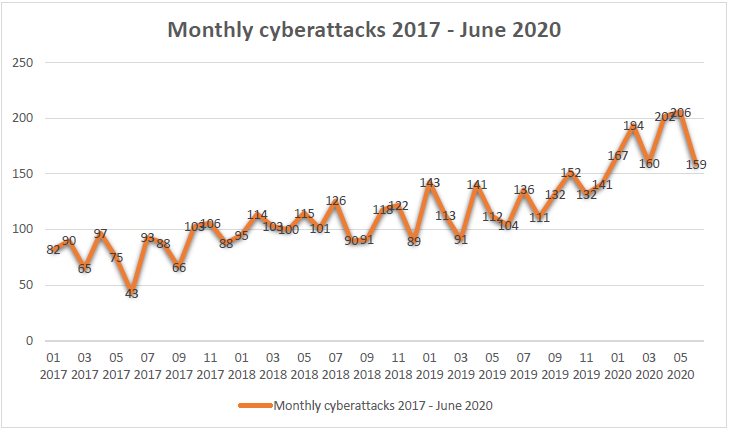
\includegraphics[width=0.5\textwidth]{graphics/threatscape_chart.PNG}
            \caption{Increasing number of monthly cyber attacks since 2017. Data is compiled from \cite{pt_threatscape_2018}, \cite{pt_threatscape_2019}, \cite{pt_threatscape_2020} and              \cite{pt_threatscape_2020q2}.}
            \label{fig:no_attacks_evolution}
        \end{figure}
		
        Concurrently, Android app security is not improving. A study conducted on over 400,000 APKs released between 2010 and 2016 belonging to over 28,000 apps analyzed how security has evolved over time \cite{android_vulnerabilities_evolution}. It discovered that critical vulnerabilities of various types have always been common in apps. Moreover, app updates generally do not improve security, and can even re-introduce previously fixed vulnerabilities. This is the largest and most comprehensive study to date. Another study found that the proportion of malware has dropped significantly in 2017 compared to 2014 \cite{newer_android_vulnerabilities_evolution}, though it studied fewer APKs than \cite{android_vulnerabilities_evolution}.
		
	\section{Motivations}
	    \label{sec:intro_motivations}
	    
	    We chose to explore Inter Component Communication vulnerabilities in Android for reasons based on the current state of mobile application security and how this vulnerability category is touched upon in related work.
	    
	    \subsection{ICC-related vulnerabilities in current mobile apps}
	        \label{subsec:ICC_vulnerabilities_current_apps}
	    
    	One of the categories of vulnerabilities that the authors of \cite{pt_mobile_apps_2019} analysed was Inter Component Communication vulnerabilities. Android components are the logical building blocks of an app, and components can communicate with other components, of the same app or of other apps on the same device.
    	
    	In the study conducted in \cite{pt_mobile_apps_2019}, 29 percent of client apps used insecure inter-process communication, and the average Android app had 1.1 ICC-related vulnerabilities \cite{pt_mobile_apps_2019}. Insecure inter-component communication is a high-risk vulnerability, and it is more dangerous than insecure storage or other common vulnerabilities \cite{pt_mobile_apps_2019}, and therefore deserves attention from developers and cyber security specialists.
		
		Moreover, while the overwhelming majority of vulnerabilities of other types are introduced in apps through the use of third-party libraries and rarely through developer code, ICC vulnerabilities differ in this regard. According to \cite{android_vulnerabilities_evolution}, between a third and a half of ICC vulnerabilities come from code written by the developer directly. Therefore, education regarding this type of vulnerability addressed to the average developer would greatly help with minimizing the occurrence of these faults.
		
		Finally, the reality is that software developers are not always trained in cybersecurity, may lack costly automatic analysis tools, or do not have the time to design and implement secure software due to tight deadlines \cite{malwarebytes_blog}. Therefore, there needs to be more awareness of cyber security in the software development industry, especially among developers.
		
		\subsection{ICC-related vulnerabilities in related work}
		    \label{subsec:ICC_related_work}
		
		Vulnerabilities and cyber attacks concerning communication between Android components are not showcased in detail or intuitively in real-world projects similar to mine.
		
		Damn Insecure and Vulnerable App has challenges 9 and 10 that show examples of hijacking intents meant for a vulnerable activity. DIVA also contains challenge 11 where a malicious user can send intents to extract data from an unprotected content provider \cite{diva_walkthrough}. 
		
		Purposefully Insecure and Vulnerable Android Application, also called PIVAA from here on, has three challenges on components that are insecurely exported and thus can be sent malicious intents. The challenges show this vulnerability in a broadcast receiver, a service, and a content provider, respectively.
		
		Another intentionally insecure Android app used for educational purposes is InsecureBankv2 \cite{android_insecure_bank_github}. Similar to PIVAA, it contains vulnerable components that can be started by a malicious app with a specially crafted intent, though it has a vulnerable activity, broadcast receiver, and content provider and no service, unlike PIVAA \cite{android_insecure_bank_walkthrough}. Furthermore, another ICC-related vulnerability it contains is intent hijacking, which allows malware to intercept intents sent by components of the vulnerable app.
		
		Damn Vulnerable Web Application, an intentionally insecure web application with vulnerabilities such SQL injection or Cross-Site Scripting, does not cover any Inter Process vulnerabilities. TryHackMe.com is an interactive website for learning cyber security and penetration testing. Although easy to use and very useful, it has no dedicated activities on Android ICC.
		
		None of the projects mentioned in this subsection cover all types of ICC vulnerabilities. Furthermore, DIVA, PIVAA, and InsecureBankv2 only offer one application that has various components for each vulnerability they implement, they do not offer standalone apps for each vulnerability. More importantly, these applications need to be used together with ADB shell on a computer to perform each attack. Thus, these projects do not offer real examples of malicious apps. On top of that, they provide little to no instructions and do not show detailed explanations and code examples of the vulnerability and how to fix it. Finally, they do not provide much interactivity and some of the apps contain major UI bugs, such as the About project activity in PIVAA.
		
		Damn Vulnerable Web Application, or DVWA, had multiple security levels for each vulnerability, where in each one the vulnerable program uses increasingly secure code. It tells the user what each level does, how secure it is, and shows relevant source code for it. This is a very useful feature that is not shared by the three insecure Android app projects mentioned earlier in this subsection.
		
	\section{Project Aims and objectives}
		\label{sec:intro_objective} 
    	
    	This project aims to create an educational tool that explores vulnerabilities related to insecure Inter Component Communication in Android, that can be used by penetration testers and developers. This tool should teach users about ICC vulnerabilities and attacks in Android apps and raise awareness.
        
        The primary objectives of the project, that make up the minimal viable product, are:
        
        \begin{itemize}
            \item Develop a home application through which the user can access all educational material and can interactively learn about each vulnerability and how to exploit it and fix it.
            \item Develop a series of apps that act as either a vulnerable app or a malicious app. Each challenge has two apps, a vulnerable app and a malware that exploits the former.
            \item Make sure that the experience of using the product is cohesive and pleasant.
        \end{itemize}
	
	\section{Contributions} 
		\label{sec:intro_contributions} 
		
		The main contributions of this project are as follows:
		
		\begin{itemize}	
		
			\item \textbf{An intentionally insecure Android image focused on Inter Component Communication vulnerabilities and attacks}
			
			\item \textbf{An educational tool for Android vulnerabilities that does not require the use of ADB shell and can be used on one's smartphone}
			
			\item \textbf{An intentionally insecure Android image which includes malware:}
			Unlike existing projects of this type, we have developed real malware apps that attack other apps in the image.
			
			\item \textbf{An intentionally insecure Android image with multiple security levels for each vulnerability, like DVWA has:}
			No other related work on Android except ours implements this, to our knowledge.
			
		\end{itemize}
	\chapter{Background}
    \label{chap:background}

   This chapter will cover the necessary technical background regarding Inter Component Communication. We will explain what components, manifests and permissions are in Android, discuss how components communicate between each other and explore the two major types of Inter Component Communication attacks.
    
    \section{Android Components}
        \label{sec:android_components}
        
    Android mobile apps are made up of logical building blocks called components. A component is an entity which allows the user or the operating system to access the application \cite{android_app_fundamentals}. Therefore, a component does not necessarily correlate with other computing concepts such as processes or threads. There are four types of components in Android: activities, services, broadcast receivers and content providers. We will detail these in the rest of section \ref{sec:android_components}
        
    \textbf{Activities} represent the individual app UI screens through which a user interacts with the app. For example, a news aggregator application might have an activity for viewing a list of news articles. Activities are used by the operating system to keep track of what the user sees on screen, what information they are interested in, and the information of minimized apps that might be needed later \cite{android_app_fundamentals}.
        
    \textbf{Services} are components used for running long-term operations in the background. Importantly, a service does not represent a separate process or thread, but an interface for the system to let the app work in the background \cite{whats_is_a_service}. A service does not have a user interface itself. Examples of the usage of services include VPN apps that maintain a VPN connection in the background.
    
    There are three types of services: foreground services, which perform tasks that are noticeable to the user and must display a notification, background services, which do things that are not noticeable to the user, and bound services, which act as servers responding to requests made by client components \cite{services_overview}.
        
    \textbf{Broadcast receivers} are components used to receive system wide broadcasts. These broadcasts are messages sent by the operating system or by other apps. Applications can react to various events by using broadcast receivers. For example, the system can send a broadcast to let apps know that the device’s battery is low. An app can use a receiver to listen for an event even when the app is not running. Receivers do not have a user interface but can display notifications. In addition, it is worth noting that they do not have to be declared in the manifest but can be created programmatically as well. 
    
    There are three types of broadcasts, two of which are relevant to our project:
    \begin{itemize}[noitemsep]
        \item \textbf{Normal broadcasts} are sent to all receivers at the same time, and each receiver can react independently of other receivers.
        \item \textbf{Ordered broadcasts} are sent to receivers one at a time. Unlike with a normal broadcast, the receiver currently processing the broadcast can change what information the broadcast contains, and can even cancel the broadcast, so that it will not be sent to further receivers \cite{broadcasts_overview}. Broadcast receivers can be registered with a certain priority for getting broadcasts.
    \end{itemize}
        
    \textbf{Content Providers} are interfaces through which apps can access data stored in persistent storage such as a remote server, an SQL database or local file storage. A provider can be used by components of the same app or by components of other apps. Therefore, they are used by the system to manage access to shared data. Content providers can restrict access to the data to apps with certain permissions and give temporary access to certain files only \cite{android_app_fundamentals}.
    
    The manifest of an Android app is an XML file that gives the system information about the app’s structure, capabilities and needs. All app components, except broadcast receivers, need to be declared in the manifest file, and for each component you can define permission requirements and the capabilities of the component \cite{android_app_fundamentals}. Moreover, the developer can say in the manifest file what hardware or software system features the app uses. For example, an app would not be installed on a device if its manifest said it required a microphone and the mobile device did not posses microphone hardware. Permissions are explained later in section \ref{sec:permissions}.
    
    \section{Permissions}
        \label{sec:permissions}
        
    Android follows the principle of least privilege. This principle is enforced through a system of permissions, meaning that an application can only access sensitive data, system features or components of other applications if it possesses the necessary requirements \cite{permissions_guide}. For instance, an application needs the correct permission to access the user’s contacts. 
    
    There are four types of permissions, based on their protection level, three of which are relevant to this project:
    \begin{itemize} [noitemsep]
        \item \textbf{Normal permissions} are for unimportant resources, such as the permission to set the time zone \cite{permissions_guide}. They are granted automatically at install time.
        \item \textbf{Dangerous permissions} are for important resources such as private user information, or that can affect the state of the system or of other apps. The user needs to give explicit permission in the app to utilise these resources.
        \item \textbf{Signature permissions} are special permissions designed for use among a group of apps created by the same developer. An app is automatically granted a signature permission at install time only if it is signed by the same certificate as the app that defined the permission. The certificate can be self-signed by the developer. Its purpose is to identify the author of an app \cite{define_custom_permission}.
    \end{itemize}
    
    Moreover, developers can protect a component of an app with permission requirements by adding an \lstinline|android:permission| tag in the manifest file. Only components in apps that have that permission will be able to send an intent to the protected component.
        
    Applications can declare their own permissions. These can be used to restrict access to components of an application, or protect broadcasts of that app. This is done by declaring a permission in the manifest file of the app, as you can see in listing \ref{lst:custom_permission}.
    
    \lstinputlisting[language={xml}, label={lst:custom_permission}, caption={A declaration of a custom permission in the manifest of the News Aggregator app of this project.}]{./listings/custom_permission.xml}
    
    \section{Inter Component Communication}
        \label{sec:inter_component_communication}
    
    By default, each Android application runs in its own sandbox, and can not see what other applications are doing \cite{android_app_fundamentals}. Sometimes, we need the system to communicate with the apps, and applications can enrich the user's experience by collaborating. For example, a browser lets you select which social media or messaging app to use for sharing a link.
    
    Intents are a class in the Android API that are used as messages for communication between application components. Intents are used to start new activities, start and stop services, bind or unbind a component to a service, and they also represent the broadcasts that are sent to receivers. Intents can carry data in the form of a URI, as well as other data in the form of key value pairs \cite{intents}.
        
    By default, app components are not accessible to outside apps through intents. However, \textbf{exported components} can receive intents from other applications. To export a component, you can set the \lstinline|<exported>| tag in a component in the app’s manifest to true. However, if the component has an intent filter defined in the manifest, the component will become automatically exported unless the exported tag is explicitly set to false. Intent Filters will be fully explained in subsection \ref{subsec:implicit_intents}.
    
    \subsection{Explicit Intents}
        \label{subsec:explicit_intents}
        
    Explicit intents directly specify the application that should receive the intent and handle it. This is done by setting the package name of the receiving app or the full name of a component of said app \cite{intents_and_intent_filters}. In Listing \ref{lst:explicit_intent}, you can see an explicit intent sent from the Santander app of this project to an activity of the same app. The intent also contains data in the form of a URI.
    
    \lstinputlisting[language={java}, label={lst:explicit_intent}, caption={Kotlin code from the Santander app to make an explicit intent, add data to it and start an activity with it}]{./listings/explicit_intent.kt}
    
    With an explitivt intent, only the targeted component can receive the intent. Explicit intents are usually used for communication between components of the same app, such as when one activity starts another when the user clicks a button. That being said, explicit intents can be used to start components of other apps as well, if those components are exported.
    
    \subsection{Implicit Intents and Intent Filters}
        \label{subsec:implicit_intents}
        
    Unlike explicit intents, implicit intents do not directly specify what application or component it should be sent to. Instead, the Android system decides who to send it to based on the information in the intent and what other components have declared they can handle. You can see in Listing \ref{lst:implicit_intent} that the implicit intent does not specify a specific component, but specifies an action and category instead
    
    A component defines what intents it can handle by specifying Intent Filters in the manifest file. An Intent Filter defines the type of intents an application can handle. A filter can say what actions the component can perform, what intent categories it accepts, the MIME data types it accepts or the kind of URI resources it can handle. You can see an example of this Listing \ref{lst:intent_filter}. A component may declare multiple Intent Filters, and it is recommended that this is done for each task the component can do \cite{intents_and_intent_filters}.
    
    \lstinputlisting[language={xml}, label={lst:intent_filter}, caption={Declaration of an activity in the Santander app with an intent filter that the intent in Listing \ref{lst:implicit_intent} will match.}]{./listings/intent_filter.xml}
    
    \lstinputlisting[language={java}, label={lst:implicit_intent}, caption={Kotlin code from the Santander app of this project to make an implicit intent, add data to it and start an activity with it.}]{./listings/implicit_intent.kt}
    
    When an implicit intent is sent, the Android System compares its attributes against all intent filters of all components. For the intent to be matched with a filter, three tests are performed: the Action, Category test, and Data tests \cite{intents_and_intent_filters}. To pass the Action test, the Intent’s action must be amongst the actions of the filter. It passes the Category Test if all of its categories are found in the filter’s declaration, and the Data Test is passed if the data URI or MIME type matches one of the data elements in the filter. If the component has multiple filters, the intent only needs to match one for the component to receive it.
    
    If only one intent filter matches the implicit intent, Android will start that filter’s component automatically. However, if there are multiple activities that match, a dialog will be displayed to the user so they can manually select the component to handle the intent. For example, if the user clicks on a web link in an app, they might then see an Android dialog for choosing what browser to use to open that page.
    
    \section{Inter Component Communication Vulnerabilities and Attacks}
        \label{sec:icc_vulnerabilities_and_attacks}
        
    In this section, we will explain the two major types in cyber attacks concerning Inter Component Communication: \textbf{Intent Hijacking} and \textbf{Intent Spoofing}.
        
    The Android documentation recommends that explicit intents are used for intra-app communication, and implicit intents for inter-application communication \cite{intents_and_intent_filters}. However, developers sometimes use implicit intents to start a component within the same app. An attacker can make a component in the malware with an intent filter designed to match with said implicit intents, which may direct the intent to the malware. The process in which an intent is matched against a filter is described in section \ref{subsec:implicit_intents}. When receiving an intent, the component can read all of its data. Therefore, even if the implicit intent is meant for external use, if it has sensitive information in it, that data could be intercepted. In general, vulnerabilities Intent Hijacking attacks are fixed by using explicit intents instead of implicit intents to send broadcasts, start activities or services \cite{2010_icc_paper}. Another way to mitigate these attacks is to not put sensitive information in implicit intents.
    
    While Intent Hijacking attacks work by accidentally sending an intent to malware, Intent Spoofing attacks happen when an exported victim component is unexpectedly activated by an attacking component using an intent. Often, this attack targets components that are not meant to be accessible outside of their apps, but because they have an intent filter and the \lstinline|<exported>| tag in the manifest is not set, they are exported automatically. Because exported components are accessible to other apps, the attacker can start them with an explicit intent. This class of attacks was originally going to be covered by this project, as mentioned in the Initial Document, but due to time constraints we have not managed to implement any challenges with Intent Spoofing attacks. We still plan to do it in the future.
    
	\chapter{The intentionally insecure app suite}
    \label{chap:implementation}

   This chapter will explain my implementation for this project. It will first give an overview of the architecture of the software product. Following that, we will show the System Requirements, explore the DVM-ICC app and then explain each challenge. Finally, we will document how testing for the project was done.

    \section{Architecture} 
        \label{sec:architecture}
        
    The central part of the software implementation consists of the Damn Vulnerable Mobile - Inter Component Communication app. This Android app contains the educational material needed to understand Android ICC and complete each challenge, encourages the user to learn interactively, provides access to each challenge and to settings to control the challenge or the learning experience. 
    
    The rest of the project consists of a series of Android apps that play the role of either a vulnerable app or a malware. These apps are made to appear to be authentic apps with real-world functionalities, though many of them are nowhere close to full-feature app. Each challenge consists of an authentic scenario of a malware app attacking one of the vulnerable apps through one particular ICC vulnerability.
    
    The DVM-ICC app communicates with the challenge apps through the use of files in order to apply various settings to control the behaviour of the apps. These settings are explained in subsection \ref{subsec:challenge_settings}. Moreover, each pair of vulnerable and malicious apps communicate between each other as a result of the cyber attack, through the medium of Intents. The manner in which this communication takes place will be explained in detail for each challenge in section \ref{sec:challenges}.
    
    \section{Functional System Requirements}
    \label{sec:requirements}
    
    % text would be too close to table caption, so i add space after it.
    \vspace{-2mm}
    This section presents the formal Functional System requirements for finished product.
    \vspace{2mm}
    
    \begin{center}
        \begin{longtable}{|p{0.4cm} |p{5.7cm} |p{6.9cm} |}
        \caption{Functional System Requirements for the project.} \label{table:requirements} \\
        
        \hline \multicolumn{1}{|c|}{\textbf{No}} & \multicolumn{1}{c|}{\textbf{Description}} & \multicolumn{1}{c|}{\textbf{Fit Criteria}} \\ \hline 
        \endfirsthead
        
        \multicolumn{3}{c}%
        {{\bfseries \tablename\ \thetable{} -- continued from previous page}} \\
        \hline \multicolumn{1}{|c|}{\textbf{No}} & \multicolumn{1}{c|}{\textbf{Description}} & \multicolumn{1}{c|}{\textbf{Fit Criteria}} \\ \hline 
        \endhead
        
        % \hline \multicolumn{3}{|r|}{{Continued on next page}} \\ \hline
        \endfoot
        
        \hline \hline
        \endlastfoot
        
         \hline
         1 & The product provides detailed explanation of the technical background needed to understand the vulnerabilities of each challenge. & The DVM-ICC app displays detailed descriptions of Android components, permissions, Inter Component Communication and of each individual attack and vulnerability. \\
         \hline
         2 & The custom Android image shall allow the user to perform the following cyber-attacks in the form of challenges: Broadcast Theft, Broadcast Theft - DOS, Broadcast Theft - MITM, Activity Hijack and Content Provider URI Hijack. & There is a vulnerable app and malware for each named challenge, and the malware can successfully attack the former. The DVM-ICC app provides guidance for identifying these apps and using them. \\
         \hline
         3 & The first task of the challenge is for the user to identify the vulnerable app and malware. & The user can view in the DVM-ICC app the manifest and intent sending code snippets for every app of the project. Based on these, they shall be able to recognise the pair of apps for each challenge and submit their answers in the DVM-ICC app. \\
         \hline
         4 & Each challenge mentioned in requirement 2 has between two and five security levels. These levels show different ways to protect an app against the attack of that challenge, each being increasingly more secure. & The user can select between 2 and five levels for each challenge. Depending on the level, the vulnerable app will use code that is less secure or more secure. The malware will be able to attack the app in all levels, except the last level, the Impossible level. \\
         \hline
         5 & The user can view information about the security levels of each challenge. & After completing the task from requirement 3, the user can view in an activity detailed descriptions for how each security level is different, along with relevant code snippets of the vulnerable app. \\
         \hline
         6 & As the second task of every challenge mentioned in 2, the user shall be able to see the result of the cyber attack. & For all security levels in the challenge, except the Impossible level, the user can view any data stolen from the vulnerable app and a flag in the malware, or observe the effects of the attack. Each level has a unique string flag, which the user needs to find and submit in the DVM-ICC app. \\
         \hline
         7 & The product will have a mode for experienced users. & The user can switch to and from the "Experienced" mode, which hides all information that would help the user and only displays code snippets. \\
         \hline
         8 & The product will have a Make Own Malware mode. & In this mode, the malware is disabled, and the user only sees an explanation of the vulnerability and attack. \\
         \hline
        \end{longtable}
    \end{center}
    
    \section{DVM-ICC Application}
        \label{sec:home_app}
        
    In this section, we will explore the features of the DVM-ICC Android app. While doing so, we will explain the intended workflow that a user needs to follow and how the app provides an educational experience. The following description applies to the Beginner mode. The app has three different operation modes, which are fully explained in subsection \ref{subsec:challenge_modes}.
    
    \subsection{Home Menu}
        \label{subsec:home_menu}
        
    The first screen the user sees when starting the app has 3 sub-pages: Introduction, Info, and Challenges, like in figure \ref{fig:home_menu}. The Introduction page gives an introduction to the project and explains the intended workflow for using the product. The Info page provides the necessary technical background to understand ICC vulnerabilities and attacks. It covers what components and permissions are, how components communicate with each other and how Intent Hijacking attacks operate. The Challenges page lets the user select what challenge they want to start, as shown in figure \ref{fig:home_menu}.
    
    \begin{wrapfigure}[17]{r}{0.32\textwidth}
        \centering
        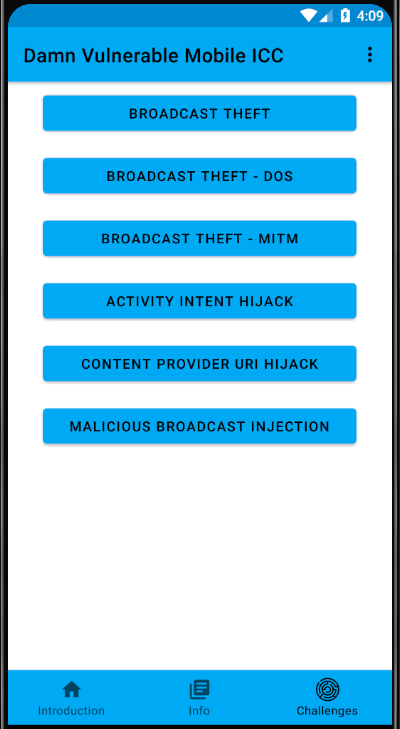
\includegraphics[width=0.32\textwidth]{graphics/home_activity.PNG}
        \caption{The first menu in the DVM-ICC app.}
        \label{fig:home_menu}
    \end{wrapfigure}
    
    \subsection{Challenge Settings}
        \label{subsec:challenge_settings}
        
    When clicking on a challenge, the user is taken to a menu where they can change the settings that define how the challenge will be undertaken. Here, you can set the operation mode for the challenge. Moreover, the user can enable or disable the malware of the selected challenge. If disabled, the malicious app will not perform any cyber-attack and therefore it will not interfere with any vulnerable app or the rest of the system.
    
    The most important setting on this screen is the security level of the vulnerable app. Inspired by DVWA, as described in subsection \ref{subsec:ICC_related_work}, these levels define how secure the vulnerable app is against cyber attacks. Each challenge's vulnerable app has between 2 and 5 security levels, with each successive level using more secure code. This culminates with the Impossible level, where the vulnerability is fixed and the malware can not perform the attack. When the malware is enabled, it will overcome the defences of the current security level, except for the Impossible level. The number of security levels and their meaning depends on the challenge.
    
    These settings are written to a text file that is located on the device's external storage, where it can be accessed by other apps that are part of this project. The security level setting will dynamically change the behaviour of the vulnerable and malicious apps, and the user does not need to restart them, with some exceptions. The settings can be changed at any time while doing a challenge.
    
    \subsection{Identifying the malware and the vulnerable app}
        \label{subsec:identify_challenge_apps}
        
    Once the user applies the settings described in subsection \ref{subsec:challenge_settings}, the application starts the Challenge activity, which you can see in figure \ref{fig:manifests_fragment}. The first task of every challenge is to identify the pair of vulnerable and malicious apps for that challenge from amongst all of the apps that are part of the project, except the DVM-ICC app itself. 
    
    \begin{wrapfigure}[19]{r}{0.4\textwidth}
        \centering
        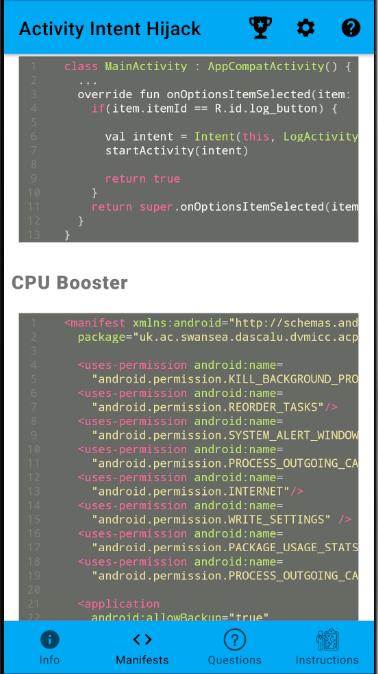
\includegraphics[width=0.4\textwidth]{graphics/manifests.PNG}
        \caption{The Manifests page in the Challenge activity.}
        \label{fig:manifests_fragment}
    \end{wrapfigure}
    
    The Info page gives a detailed description of the specific cyber attack related to this challenge. After reading and understanding this information, the user needs to go to the Manifests page, where they can view for each app the contents of its manifest and all snippets of code that sends intents, as shown in figure \ref{fig:manifests_fragment}. Based on the technical background the user was given in the Info page and the Home Menu from subsection \ref{subsec:home_menu}, they need to look through the code in the Manifests page and try to identify the vulnerable app and the malware for this challenge. 
    
    The user should be able to detect vulnerable apps by looking for intents being sent implicitly or for exported components, for example. Malwares can be usually identified by the use of intent filters matching intents that are only sent by a vulnerable app, or by sending an explicit intent to another app that is part of this project. The features that identify the vulnerable app and malware depend on the selected challenge. 
    
    The Questions page contains text boxes where the user can type in their answers and be told if they have correctly identified the apps.
    
    \subsection{Performing the cyber attack}
        \label{subsec:perform_attack}
        
    Now that the user knows the correct pair of apps for this challenge, the next task is to use these apps to witness the cyber attack take place.
    
    Once you have correctly answered the questions regarding the identity of the malware and vulnerable app, the Instructions page will display detailed instructions for using the apps such that the specific cyber attack for that challenge will take place. This page can be accessed from the activity shown in figure \ref{fig:manifests_fragment}.
    
    In general, the user is asked to take a look at the two apps to familiarise themselves with them and what they can do. Then, the user should make sure that the security level is set to low. After that, they should use the vulnerable app and malware according to the provided instructions in order to trigger the attack and observe it. 
    
    \begin{wrapfigure}[19]{r}{0.4\textwidth}
        \centering
        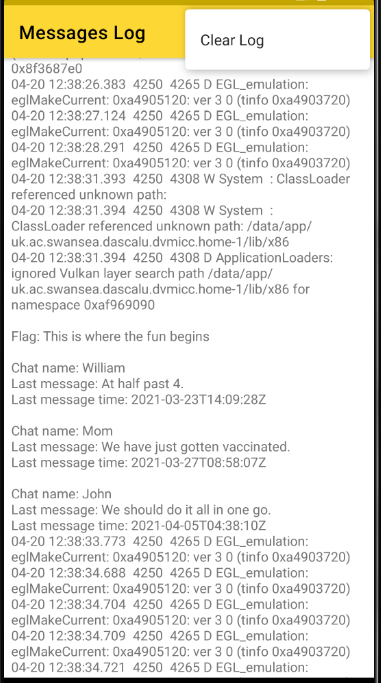
\includegraphics[width=0.4\textwidth]{graphics/log.PNG}
        \caption{Log of the malware for Content Provider URI Hijack after it successfully attacked the vulnerable app.}
        \label{fig:malware_log}
    \end{wrapfigure}
    
    Following that, the user needs to look in the malware's log, which is accessed from its app bar. If the attack was successful, the malware should have written in its log the flag associated with this specific challenge and security level, along with any relevant data it managed to steal from the vulnerable app. These would be hidden amongst the output of the Android Log of the malware. 
    
    You can see an example of this in figure \ref{fig:malware_log}, where the messages from the Whatsapp vulnerable app have been stolen by the SMS Messages malware. The user should then copy the flag and submit it to the flag question for the current security level in the Questions page in the DVM-ICC app, to prove they have completed one level of the challenge. 
    
    At this point, the user should clear the log of the malware to see the effects of the next attack more easily, and then change the security level to the next value. They should repeat the process described in this subsection for every security level of that challenge.
    
    Through performing the task described in this section, the user will witness an example of a cyber attack happening in an authentic scenario, with a real malicious app exploiting an insecure app.
    
    Once the user has performed the cyber attack and submitted the correct flag for every security level, they have completed that challenge. As a reward, they can now click on the trophy button on the app bar of the Challenge activity, seen in figure \ref{fig:manifests_fragment}. This will open an activity where the user can read the conclusion to the current challenge. This text will give a summary of the whole challenge, going through how the vulnerability is introduced, how the attacker can create malware that takes advantage of it, and how to fix the vulnerability. The purpose of this conclusion is to condense all of the information that the user should take away from this challenge.
    
    \subsection{Security Levels Explanation}
        \label{subsec:security_levels_explanation}
        
    While completing the task described in subsection \ref{subsec:perform_attack}, the user can click on the Help button at the top right in figure \ref{fig:manifests_fragment} to view an explanation of the security levels for the current challenge. This view is hidden until the user has identified the pair of apps for the current challenge, as explained in subsection \ref{subsec:identify_challenge_apps}.
    
    For each level, it will explain how it works and why it is more secure than the previous level. Following this explanation is a view of the full manifest of the vulnerable app, as it would be used for that security level. Finally, this view might show code snippets that introduce a vulnerability through the way they send an intent.
    
    \begin{wrapfigure}[20]{r}{0.4\textwidth}
        \centering
        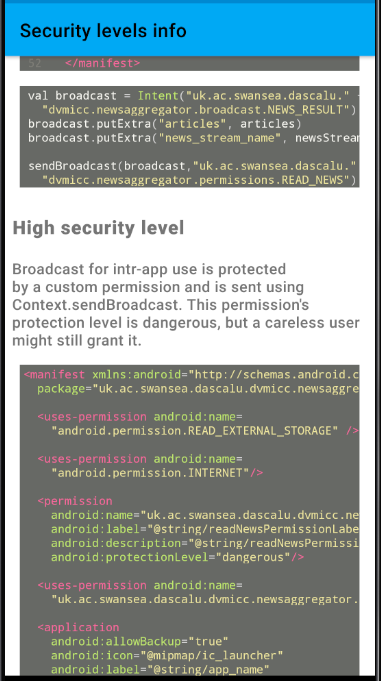
\includegraphics[width=0.4\textwidth]{graphics/security_level_explanation.PNG}
        \caption{Part of the explanation of the security levels for the Broadcast Theft Challenge.}
        \label{fig:security_levels}
    \end{wrapfigure}
        
    You can see part of the Security Levels explanation for the Broadcast Theft challenge in figure \ref{fig:security_levels}, as an example. The top code snippet shows the code used to send a broadcast in the News Aggregator app in the Medium security level. Since this code sends the broadcast implicitly, it is insecure.
    
    This activity teaches the user how and where the vulnerability is introduced and what steps a programmer can take to secure the vulnerable app, complete with code examples from the app itself. Some solutions fail to completely remove the vulnerability, and this activity teaches the developer why they are inadequate. The explanation of the Impossible level shows how to completely remove the attack surface.
    
    By looking at these explanations while performing the task described in subsection \ref{subsec:perform_attack}, the user can see how the cyber attack of that challenge can still succeed despite the programmer implementing some security defences.
    
    \subsection{Operation Modes}
        \label{subsec:challenge_modes}
    
    As mentioned at the beginning of section \ref{sec:home_app}, the DVM-ICC application supports three modes. The Beginner mode has already been described in sub\cref{subsec:home_menu,subsec:challenge_settings,subsec:identify_challenge_apps,subsec:perform_attack,subsec:security_levels_explanation}. It is meant for less experienced users, who need to be given detailed explanations for each vulnerability.
    
    The Expert Mode works in the same way as the Beginner mode, but it hides a lot of information to increase the difficulty. In the Challenge activity from figure \ref{fig:manifests_fragment} on page \pageref{fig:manifests_fragment}, the Info page will be hidden, and the Security Levels Explanation activity from figure \ref{fig:security_levels} will only contain code snippets, without any explanations.
    
    The Make your Own Malware mode disables the malware app of the current challenge in order to allow the user to create their own malware and attack the vulnerable app without interference from the included malware. In this mode, the user only has access to the Info page described in subsection \ref{subsec:identify_challenge_apps} and the Security Levels activity described in subsection \ref{subsec:security_levels_explanation}.
    
    \section{Challenges}
        \label{sec:challenges}
        
    Section \ref{sec:home_app} covered the general workflow for using the software of this project, which applies to all challenges. In this section, we will focus on the vulnerability explored by each challenge, and the pair of malware and vulnerable app that demonstrate it. All five challenges involve variations of the Intent Hijacking attack presented in subsection \ref{sec:icc_vulnerabilities_and_attacks}.
    
    For all challenges presented here, the description in the Implementation subsection of each challenge describes the interaction between malware and vulnerable app when the security level is set to Low. The other security levels are presented in the Security Levels subsection of each challenge.
    
    \subsection{Broadcast Theft}
        \label{subsec:broadcast_theft}
        
    When a broadcast is sent, the sender does not receive any indication of what components have received that broadcast. A malicious app can register a broadcast receiver with as many intent filters as possible to listen to many public broadcasts \cite{2010_icc_paper}. The malware can read the data in the broadcasts without the user knowing it, and could therefore be used as spyware. 
    
    Moreover, if an implicit intent is used to make a broadcast meant for an app’s internal use, that broadcast could be sent to any receiver on the device with a matching filter. An attacker could reverse engineer an application, see the intent filter that matches the broadcast, then add an identical filter to a broadcast receiver in their malware.
    
    \subsubsection{Implementation}
        \label{subsubsec:broadcast_theft_implementation}
        
    The vulnerable app for this challenge is News Aggregator, an application that looks for online news articles from various sources and shows them to the user. When its service has downloaded the news articles, it will send a broadcast with the JSON data, which will be received by a broadcast receiver in the app. This receiver will process the data and update the UI. The broadcast is sent as an implicit intent, and any receiver with an intent filter that includes the action of the broadcast will get it. In a real-world app, developers might use an implicit broadcast for intra-app communication to make the app more loosely coupled and more modular. Another reason might be that they want other apps made by them to know when News Aggregator has gotten some articles.

    The malware for this challenge is the Call Logger app, which displays the user's call history. In it, the attacker has added a broadcast receiver with an intent filter that is identical to that of News Aggregator's receiver. If both apps are installed on the same device, the broadcast sent by News Aggregator will be received by both its receiver and the malware's receiver. Call Logger can therefore see what news articles a user is looking at and what they might be interested in.
    
    \subsubsection{Security Levels}
        \label{subsubsec:broadcast_theft_security_levels}
    
    When sending a broadcast, the developer can specify the permission that a receiver's app needs to have to be able to get the broadcast, like in Listing \ref{lst:send_broadcast_with_permission}. This can be used to guard against Broadcast Theft. A developer can declare their own custom permission, as seen in Section \ref{sec:permissions}, which must be obtained by receivers to get broadcasts sent by the developer's app. 
    
    \lstinputlisting[language={java}, label={lst:send_broadcast_with_permission}, caption={Kotlin code from News Aggregator for sending a broadcast protected by a custom permission.}]{./listings/sendBroadcast.kt}
    
    If the developer does not set the protection level of the permission, it will default to "normal". This means that the malware will get it automatically at install time if it asks for that permission in its manifest. This is what happens in the Medium security level. In the High security level, the protection level of News Aggregator's custom permissions is set to "dangerous", meaning the malware needs to ask the user to grant that permission. This is quite secure, but a careless user may still grant it. The most secure protection level for the custom permission is "signature", but if the private key of the certificate is not stored securely, it can be stolen and be used to sign the malware, which would be able to get the permission when it is installed and receive the broadcast. This is demonstrated in the Very High security level. The protection levels of permissions were explained in Section \ref{sec:permissions} and an example was shown in Listing \ref{lst:custom_permission}.
    
    Because permissions with a normal or signature protection level are granted at install time, they can not be changed dynamically. Therefore, for the Medium and Very High security levels, the user needs to use the Call Logger 2 and 3 app, respectively. These are identical to Call Logger, except they ask in their manifest for the relevant permission for their security level, and they have a different app icon.
    
    In the Impossible security level, the broadcast is sent as an explicit intent, as the News Aggregator service sets the name of the app whose components can receive the broadcast. This completely removes the vulnerability \cite{2010_icc_paper}. However, it also means that the broadcast can not be received by other apps, which the developer might want, depending on the situation.
    
    \subsection{Broadcast Theft - Denial of Service}
        \label{subsec:broadcast_theft_dos}
        
    The challenge presented in subsection \ref{subsec:broadcast_theft} focused on normal broadcasts. Ordered broadcasts are sent to receivers one at a time, as explained in Section \ref{sec:android_components}. Using ordered implicit broadcasts can not only enable eavesdropping as described in subsection \ref{subsec:broadcast_theft}, but denial of service attacks as well \cite{2010_icc_paper}. A malicious app can register a broadcast receiver with a very high priority to ensure it is the first to receive it. It can extract the data from the broadcast, and then abort the broadcast, ensuring the intended receivers do not get it and thus perform a Denial of Service attack.
    
    \subsubsection{Implementation}
        \label{subsubsec:broadcast_theft_dos_implementation}

    The Call Redirect app is the vulnerable app for this challenge. This app redirects phone calls by automatically adding a customizable country code prefix before the number is dialed. It achieves this by having a broadcast receiver that listens for broadcasts with the action NEW\_OUTGOING\_CALL, sent by the OS whenever a call is being made \cite{intents}. This broadcast is ordered, and it contains the dialed phone number. The Call Redirect reads this number, adds the prefix, and then sets the new number to the broadcast.
    
    The malware for this challenge is the CPU Booster app, which pretends to improve the performance of the device but does not actually do anything. It will also have a receiver that listens for broadcasts with the NEW\_OUTGOING\_CALL action. This receiver will have the maximum possible priority declared in the malware's manifest. Consequently, it will get the broadcast before Call Redirect. It reads the dialed phone number, then cancels the broadcast, as seen in Listing \ref{lst:ordered_broadcast_dos}. The legitimate app's receiver will not receive it and the phone call will be canceled.
    
    \lstinputlisting[language={java}, label={lst:ordered_broadcast_dos}, caption={Kotlin code from the CPU Booster broadcast receiver for canceling an ordered broadcast.}]{./listings/orderedBroadcastDOS.kt}
    
    \subsubsection{Security Levels}
        \label{subsubsec:broadcast_theft_dos_security_levels}
        
    This challenge only has Low, High, and Impossible security levels.
        
    Since the broadcast is sent by the system and not by the app, we can not protect it with a permission. The developer of the Redirect app can set their receiver's priority to the maximum possible value as the malware does. This way, the receiver of this app will hopefully be called before the malware's receiver, change the number in the broadcast, and then cancel it so the malware does not receive it. The number will still be dialed because when the broadcast was sent by the OS, a final receiver was specified, which gets the broadcast even if it is canceled. This is what the vulnerable app does in the High security level.

    According to the Android documentation, receivers with the same priority are executed in an arbitrary order \cite{broadcasts_overview}. From our experience, on devices on Android 7.1 or 8, receivers with the same priority are called in alphabetical order of their app package names. For this reason, the package name of the malware is acpu\_booster, to maximise the chance its receiver will get called first, before Call Redirect's receiver can cancel the broadcast. Consequently, the attack can still happen in the High security level. Moreover, other legitimate receivers do not get the ordered broadcast, as Call Redirect canceled it before they had the chance to receive it.

    Therefore, the best way to fix this vulnerability rests with the user. CPU Booster can not receive the broadcast if it does not have permission to access phone calls from the user, and it has no obvious reason it would need it. In the Impossible level, the user should see that the app is suspicious and they should uninstall it or remove its permission.  
    
    \subsection{Broadcast Theft - Man In the Middle}
        \label{subsec:broadcast_theft_mitm}
        
    The vulnerability explored by this challenge is the same as the for the Broadcast Theft - DOS challenge in subsection \ref{subsec:broadcast_theft_dos}. The difference is that the cyber atack has a different outcome, it is a Man in the Middle attack instead of Denial of Service.

    This challenge's vulnerable app is Call Redirect yet again. The malware for this challenge is the Battery Booster app, which pretends to improve the battery life of the device, and yet again does not actually do anything. It will also have a receiver that listens for broadcasts with the NEW\_OUTGOING\_CALL action, in the same way CPU Booster did. It will get the broadcast before Call Redirect, read the phone number and replace it with a different phone number, then send the permission to the next receiver. The legitimate receiver will receive the broadcast with the injected number and the country code to it. This phone number will then be dialed. Battery booster can be used to stealthily re-direct phone calls to malicious phone numbers.
        
    The Security levels for this challenge are Low, High, and Impossible, and they function in the same way as the security levels of Broadcast Theft - DOS, described in subsection \ref{subsec:broadcast_theft_dos}. The only major difference is that the malware does not cancel the broadcast and instead changes its data.
    
    \subsection{Activity Intent Hijack}
        \label{subsec:activity_hijacking}
        
    In this type of attack, a hacker takes advantage of the use of implicit intents so that a malicious activity is launched instead of the intended one, by declaring a matching intent filter for their malicious activity in the manifest.
    
    In a sophisticated version of this attack, the attacker can use phishing to steal user credentials \cite{2010_icc_paper}. If an app uses an implicit intent to start its Login activity, a hacker can use an identical intent filter for a fake identical-looking Login activity in their malware. The implicit intent will match both the fake Log In activity and the legitimate one, and thus prompt the user to choose between them. The attacker can give a confusing name to their malware, or make the icons of the two apps similar, to make the user choose the malware. The unaware user then types in their credentials on the fake Login screen, which are then sent to the hacker.
    
    \subsubsection{Implementation}
        \label{subsubsec:activity_hijack_implementation}
        
    The vulnerable app for this challenge is SwanBank, a banking app. After they log in, the user can view details of fictitious bank accounts and can make fictional payments to another account, which will decrease the balance of one of the accounts displayed in the app.
    
    SwanBank has an intent filter for its Login activity, which you can see in Listing \ref{lst:intent_filter}, so that the user can click on a link that starts the app to make a payment. The link contains details of the recipient of the payment, such that these details are already filled in when the app launches and therefore making the payment easier. An implicit intent with this link can be sent from another app. It will match SwanBank's intent filter and start the Login activity to authenticate the user, before going to the payment screen.
    
    \begin{wrapfigure}[18]{r}{0.32\textwidth}
        \centering
        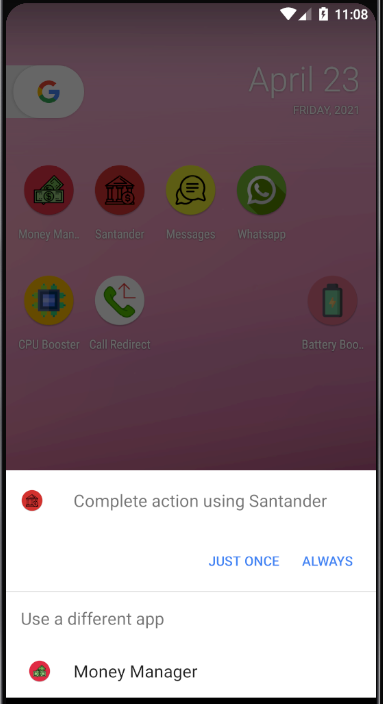
\includegraphics[width=0.32\textwidth]{graphics/activity_hijack.PNG}
        \caption{Choosing between activity of vulnerable app and malware.}
        \label{fig:activity_hijack}
    \end{wrapfigure}

    The attacker decompiled the SwanBank app to see the code for the Login activity and its intent filter. They made an activity in the Money Manager malware that looks identical to the one in SwanBank and added to it an intent filter. Money Manager is an app for tracking and categorising one's income and expenses, but it does not have full functionality.
    
    When you open the app, the user sees a Loading screen, which sends an implicit intent to start the Login activity, seen in Listing \ref{lst:implicit_intent}. There will be two filters that match with this intent, and therefore the user will be asked to pick between SwanBank and Money Manager, as you can see in figure \ref{fig:activity_hijack}. Both are financial apps, and Money Manager has a similar icon and colour theme, and therefore a careless user might select the malware. Money Manager's Login activity looks identical to SwanBank's, so the user types in their credentials, which the malware can then send to the attacker. To make it as if nothing suspicious happened, it will say the credentials are incorrect and then start the legitimate Login activity with an explicit intent.
    
    \subsubsection{Security Levels}
        \label{subsubsec:activity_hijack_security_levels}
        
    When sending intents to start an activity or service, you cannot protect them with a permission as we did with a broadcast in subsection \ref{subsubsec:broadcast_theft_security_levels}. Therefore, in the Impossible security level, the solution to fix the vulnerability is for the SwanBank Loading activity to use an explicit intent to start the Login activity, as demonstrated in Listing \ref{lst:explicit_intent}. By doing this, the intent can not be sent to the malware. Explicit intents should be used for communication between components of the same app.

    However, when the user clicks on a link in another app to make a payment, the malware's intent filter will still match that implicit intent and the attack could succeed. For this case, the solution is to use App Links such that when a user clicks on a web link, they are either taken to a web page in a browser or they are taken to an activity in your app \cite{android_app_links}. These are not implemented in the SwanBank app at the current moment.
    
    \subsection{Content Provider URI Hijacking}
        \label{subsec:provider_uri_hijacking}
        
    In section \ref{sec:inter_component_communication} we saw that intents can transmit data using a URI. These URIs can point to data stored using a Content Provider. When declaring a Content Provider in the manifest file, the developer can set the \lstinline|android:grantUriPermissions| tag of the \lstinline|<provider>| element to true. This means that the content provider can allow temporary access to data linked to in a URI in an intent for a component in another app that received that intent. Therefore, external apps can access the content, even if the provider is not exported and thus not normally accessible by external apps.
    
    To do this, the intent that transmits the URI link must have the \lstinline|FLAG_GRANT_READ_URI_PERMISSION| or \lstinline|FLAG_GRANT_WRITE_URI_PERMISSION| flags added to it. If this intent is implicit and is intercepted by a malicious component, then that component can read the data and perhaps modify it.
    
    \subsubsection{Implementation}
        \label{subsubsec:provider_uri_hijack_implementation}
        
    The vulnerable app for this challenge is Whatsapp, an internet messaging app named after the popular real-world app. This app lets you view some hard-coded chats, it does not have real functionality. These chats are accessed by the app through its content provider, which is not exported, but that has \lstinline|android:grantUriPermissions| set to true in its manifest. The user can click on a button to go to another activity where they can select what chats they want to delete. When they click the delete button, the activity will send an implicit intent that contains the selection of chats, a URI to where chats are stored in the provider, and flags for temporary read and write permissions. This intent is received by a service of Whatsapp, which is responsible for accessing the provider and deleting the messages.
    
    Because this intent is implicit, it can be intercepted by the malware, which is the SMS Messages app in this case. This app only reads SMS messages on the device, it can not send new messages. The malware contains a service with an intent filter identical to that of the Whatsapp service. The malicious service will get the intent, and because the intent has temporary access flags, the malicious service can query the Whatsapp content provider and read messages. You can see these messages in the malware's log in figure \ref{fig:malware_log} on page \pageref{fig:malware_log}. Because Whatsapp's provider is not exported, if the malware queried the provider without having that intent, an exception would be thrown.
    
    \subsubsection{Security Levels}
        \label{subsubsec:provider_uri_hijack_security_levels}
        
    This challenge only has Low, High, and Impossible security levels. In the High level, the provider is not exported and has not enabled temporary permissions overall. However, temporary permissions are enabled only for the path where chats are stored. Although the rest of the data in the provider can not be accessed by other apps, the data in this path can still be accessed by any component with a temporary permission. The temporary permission is still transmitted through the implicit intent sent by the Delete activity in Whatsapp.
    
    In the Impossible level, the intent sent by the Delete activity, which contains URIs to messages and has temporary permission flags, is sent explicitly. The Messages malware can not get these intents and therefore can not get permission to access the provider. If it tries to query the provider, an exception will be thrown.
    
    \section{Testing}
        \label{sec:testing}
        
    The testing for the project was done using manual acceptance tests, which are documented in table \ref{table:tests}. These tests consist of using the apps of the project as the final user would and observing if the software behaves as expected. They check to see that the software fulfills the System Requirements. They were conducted on both a Pixel 3 emulator with Android 7.1 and a Huawei P10 Lite with Android 8.0. All tests passed.
    
    We chose to do the tests manually instead of automating them due to time constraints and technical reasons. The project was behind schedule, and writing automated systems tests would have taken the time that was used to implement more features and challenges. Moreover, to test the communication between malware and vulnerable app, we would need to test if an intent sent by an app is received by a specific app. It is possible to test that an app sends certain intents \cite{testing_intents}, but we have not been able to find a way to test that a certain app receives the intent. Finally, the product is not complex enough to make manual testing impractical.
    
    In table \ref{table:tests}, the tests with a number followed by a "*" are a set of tests, one for each challenge, but they are grouped to save space. The correct answers for each question are defined in an xml file for each challenge. The steps and outcome of test sets 14 and 15 follow the challenge descriptions from section \ref{sec:challenges}.
    
    \begin{center}
        \begin{longtable}{|p{0.4cm} |p{5.2cm} |p{7.4cm} |}
        \caption{Manual acceptance tests related to the DVM-ICC app in general.} \label{table:tests} \\
        
        \hline \multicolumn{1}{|c|}{\textbf{Test}} & \multicolumn{1}{c|}{\textbf{Steps}} & \multicolumn{1}{c|}{\textbf{Expected Outcome}} \\ \hline 
        \endfirsthead
        
        \multicolumn{3}{c}%
        {{\bfseries \tablename\ \thetable{} -- continued from previous page}} \\
        \hline \multicolumn{1}{|c|}{\textbf{Test}} & \multicolumn{1}{c|}{\textbf{Steps}} & \multicolumn{1}{c|}{\textbf{Expected Outcome}} \\ \hline 
        \endhead
        
        \hline \multicolumn{3}{|r|}{{Continued on next page}} \\ \hline
        \endfoot
        
        \hline \hline
        \endlastfoot
        
         \hline
         1 & Open the app. & On the first menu, you can scroll through the Introduction and Info pages. \\
         \hline
         2 & Open the app and click on the Challenges button. & The Challenges page has five buttons with the texts: Broadcast Theft, Broadcast Theft - DOS, Broadcast Theft - MITM, Activity Intent Hijack, and Content Provider URI Hijack. \\
         \hline
         3 & In any challenge, go to the Manifests page. & The Manifests page contains the correct Manifest and intent sending code snippets for every app in the project. \\
         \hline
         4 & In any challenge, click on the help icon. & No new activity opens and a warning appears. \\
         \hline
         5 & In any challenge, click on the Instructions button. & Instructions page says that instructions are not available yet.\\
         \hline
         6 & In any challenge, click on the Questions button, answer the first two questions correctly then click on the Help button. & The Security Levels info activity starts. It contains the correct explanation, manifest and relevant code snippets for all security levels of the selected challenge.\\
         \hline
         7 & In any challenge, click on the Questions button, answer the first two questions correctly then click on the Instructions button. & The Instructions page displays the correct instructions for completing that challenge.\\
         \hline
         8 & In any challenge, click on the Questions button, answer all but one question correctly then click on the Trophy button. & The Challenge Conclusion page opens, but tells you to complete the challenge to unlock the conclusion.\\
         \hline
         9 & In any challenge, click on the Questions button, answer all questions correctly then click on the Trophy button. & The Challenge Conclusion page opens and it shows an explanation and commentary for the chosen challenge.\\
         \hline
         10* & In all challenges, go to the Info page. & The Info page has the correct description for the attack and vulnerability of the selected challenge. \\
         \hline
         11* & In all challenges, click on the Questions button. & The Questions page contains two questions for identifying the vulnerable app and malware, respectively, a question for the flag of each security level of the challenge, except the impossible level, and two questions for identifying the lines of code that introduce the vulnerability and attack, respectively. \\
         \hline
         12* & In all challenges, click on the Questions button. Type in wrong answers for all questions and click each submit button. & The submit buttons do not change. All question inputs are still enabled and their border turns red. \\
         \hline
         13* & In all challenges, click on the Questions button. Type in the correct answer for the selected challenge for all questions and click each submit button. & The submit buttons become outlined, their border and text are green, their text is "Completed" and they are not clickable anymore. The question inputs can not be re-edited and the correct answers can still be seen. \\
         \hline
         14* & In all challenges, for any security level, disable the malware and clear its log. Use the apps according to the challenge's instructions. & The log of the malware is still empty. \\
         \hline
         15* & In all challenges, for all security levels, enable the malware and clear its log. Use the apps according to the challenge's instructions. & The log of the malware contains the correct flag for that security level, as well as any data stolen from the vulnerable app. There may be other expected outcomes in regards to how the malware or vulnerable app behaves, depending on the challenge and the security level.\\
         \hline

        \end{longtable}
    \end{center}
	\chapter{Finding and citing resources}
	\label{chap:resources}
		
	The university has subscriptions to a vast number of major academic journals spanning a wide range of subject areas. By accessing the internet from a university network connection (Eduroam or Ethernet), the paywalls of many journals will simply vanish without any need for login credentials.

	\section{Tunnel your internet connection via the university internet}
		When you are working from outside of the university then connecting to an on campus machine via remote desktop (RemoteDesktopProtocol, TeamViewer, ect) or via port forwarding (ssh, ssh tunnel, ect) can allow you to access papers that would otherwise be behind a paywall. 
		
		If you do not have individual access to a machine that is exposed for ssh on the university network you can always use the computers in Linux Lab CF204\footnote{One caveat of using computer lab machines for remote tunnelling is that a environmentally conscious student who has worked late in the computer lab might choose to switch off the machine you were using...} for the purpose of setting up an ssh port tunnel to proxy your internet through. These machines have fixed IPv4 addresses and respond to ssh using your student account credentials. While in use your internet will be routed\footnote{Painfully slowly.} to the university and then out to the internet, granting you transparent access to journals without a paywall.

	\section{Practice your Google Fu}
		\label{sec:google_fu}
		The internet is big \cite{sizeofinternet}. Knowing how to phrase a question to a search engine is therefore an invaluable skill. If the request is simple enough, even a poorly structured query will likely return usable results. For more difficult to find resources you can leverage the language of the search engine to gather relevant papers and resources for your research more efficiently. 
		
		% An example of how to center a passage of text, control local fontsize, 
		% and create a properly formatted and clickable URL.
		\begin{center}
		{\small \url{https://www.gwern.net/Search}}
		\end{center}
		
		``Internet Search Tips'' \cite{gwern} provides an excellent review of methods and tips for scouring the internet for hard to find resources. You will also be less likely to get caught behind journal paywalls when working remotely without a tunnel as your queries can be made to look for raw pdfs that are often released by the authors directly.
			
	\section{Organizing your citations in BibTeX}
		\label{sec:resources_bibtex}
	
		BibTeX is a language for specifying resource citations. Every time you access and read an academic paper, take code from an online repository, or source the media such as images from existing works you should create a BibTeX entry in a file that you keep throughout your research. Software such as Mendeley \cite{mendeley} can help automate the process of building your BibTeX library of citations. 
		
		\lstinputlisting[label={lst:bibtex}, caption={An example BibTeX entry for an academic paper published in conference proceedings \cite{kaj86}.}]{./listings/example_bibtex.bib}
		
		The BibTeX code listing above (listing \ref{lst:bibtex}) shows an example of how to cite an academic paper, in this case one of the central papers in Computer Graphics research. The key \textbf{kaj86} is an arbitrary name chosen as a meaningful identifier for the resource. In the document text we can call on this resource as an inline citation using the LaTeX command \lstinline|\cite{kaj86}| which produces \cite{kaj86} at the location it is called. As long as a citation has been used at least once somewhere within the document then a formatted full citation will be created in the bibliography at the end of the document with the same citation number that is shown inline.
		
		It is considerably easier to be disciplined in methodically taking note of the resources you access and make use of as you access them, than it is to try and hunt them all down again at the time you need to write about them in your document. Invest time in being organized and consistent up front and it will be easier when you come to write up.
		
	\section{Properly using and formatting citations within the text}
		Usually you would not put the URL of the resource you are citing directly in the text like is done previously in section \ref{sec:google_fu}. The citation for the resource \cite{gwern} is sufficient to reference it within the text given that full details of its location are then kept neatly within the bibliography at the end of the document. 
		
		In normal usage the purpose of a citation is not to direct the reader away from your thesis, but to justify and back up assertions you are making about the state of the domain. If a reader questions your assertions then they can follow the rabbit hole of papers which will likely also make and justify assertions with even earlier papers from the literature. 
		
		In the above case the intention is for the reader of this template to actually go to that resource and read what it has to say directly. The link is therefore shown clearly within the main text to indicate that the reader should visit it. This as opposed to wanting the reader to purely acknowledge that the facts which are within the resource legitimize the points made in this document, in which case a simple inline citation is the best way to back up your assertions. Section \ref{sec:typesetting_figures_citation} specifically touches on the best practice for how to cite images which you are importing from existing work. 
	\chapter{Typesetting your thesis}
	\label{chap:typesetting}
	
	This document is intended as both a LaTeX thesis template and as a tutorial on structuring and typesetting your thesis in the LaTeX programming language.
	
	The following are some powerful online resources for learning about LaTeX:
	
	\begin{description}	
			
		\item[$\bullet$ Overleaf Documentation for LaTeX]\hfill
		
		Overleaf \cite{overleafdocs} is an online browser-based LaTeX IDE which stores your document in the cloud and provides live recompilation as you type. The documentation on Overleaf's website has a good knowledge base of examples for how to typeset things cleanly and simply in LaTeX code. 
		
		\noindent See: {\small \url{https://www.overleaf.com/learn}}
		
		\item[$\bullet$ TeX StackExchange, the StackOverflow site dedicated to TeX questions]\hfill
		
		TeX StackExchange \cite{texstackexchange} is sub-community of the StackOverflow network dedicated to questions about the TeX family of typesetting tools including LaTeX, BibTeX and others. A vast majority of the time it is unlikely that the question or issue you are facing is one that has not been encountered before, and this site more than likely to be able to point you in the correct direction. 
		
		\noindent See: {\small \url{https://tex.stackexchange.com}}
		
	\end{description}
	
	\newpage 
		
	\section{Referencing items within this document}
		In section \ref{sec:resources_bibtex} we saw examples of how to typeset citations for resources we had stored in an external BibTeX file. However, often we would like to accurately refer to the location of a resource or region of text stored somewhere else within this document\footnote{Like at the beginning of the last sentence when we referred to section \ref{sec:resources_bibtex}.}. To do this we need to annotate our LaTeX code with \lstinline|\label{key}| statements which will take on the numeric (or otherwise formatted) identifier for the current chapter, section, figure, table, equation, ect where they are directly defined. To insert an inline reference to the label you can use the \lstinline|\ref{key}| command which works similarly to the \lstinline|\cite{key}| used for external references. In the event we chose to reorder or add additional content to the document, which would change the section numbering, the document will still compile to a pdf with the correct references inserted for each \lstinline|\ref{key}| command.
		
	\section{Equations}
	\label{sec:typesetting_equations}
	
	Typesetting equations is one of the things that LaTeX does best. It has packages for different fonts and symbols for many different mathematical notations. However, to person learning how to typeset in LaTeX for the first time it can be a daunting and unwieldy user experience. Almost all LaTeX packages have documentation available in pdf format online, and documentation for packages specifically relating to fonts and symbols usually have tables enumerating the names and codes for all of the fonts symbols, organized by intended usage. 
	
	\subsection{Inline equations}
	
	Small equations like $x = 0$ can be written directly within the text by using LaTeX's maths mode shorthand controlled by dollar signs \lstinline|$ math mode $|. As long as it is not becoming cumbersome to the reader, equations such as $\mathbb{P}({A} \cap {B}) = \mathbb{P}({B} \cap {A})$ are quite neatly displayed in this fashion. 
	
	\newpage 
	
	\subsection{Block equations}
	
		For long equations it is best to provide a break in the main text of the document and format the equation using a \lstinline|\begin{equation}...\end{equation}| environment. 
		
		\begin{equation} \label{eq:veclen}
			\left\lvert a \right\rvert = \left\lvert \left[\begin{array}{c} a_0\\ a_1\\ \vdots\\ a_n\end{array}\right] \right\rvert = \sqrt{a_0^2 + a_1^2 + \hdots + a_n^2}
		\end{equation}
		
		Equation \ref{eq:veclen} demonstrates formatting a larger equation and uses an \lstinline|\begin{array}...\end{array}| environment to structure a column vector of sub-equations. Block equations should be located at a relevant point directly as they are being referred to in the text. When referred to from other locations in the document you should use the \lstinline|\ref{key}| command to insert the correct equation number.
		
		\subsubsection{Aligning multi-line block equations}
		
			When equations become even larger they may need cross over multiple new lines. When this happens it is desirable to align relevant parts of the equation on each line to one another for aesthetic reasons and to help imply structure to the reader. 
		
			\begin{equation} \label{eq:rendering_equation}
				\begin{split}
					\mathcal{L}_o\left(x, \omega_o, \lambda, t\right) &= \mathcal{L}_e\left(x, \omega_o, \lambda, t\right)\\
					&+ \int_\Omega f\left(x, \omega_i, \omega_o, \lambda, t\right) \mathcal{L}_i\left(x, \omega_i, \lambda, t\right) \left(\omega_i \bullet n\right) d\omega_i\\
					&\text{where} \quad \mathcal{L}_i\left(x, \omega_i, \lambda, t\right) = \mathcal{L}_o\left(x^\prime, -\omega_i, \lambda, t\right)\\
				\end{split}
			\end{equation}
			
			Equation \ref{eq:rendering_equation}, known as Kajiya's Rendering Equation \cite{kaj86} demonstrates the use of the \lstinline|\begin{split}...\end{split}| environment which uses a single un-escaped \& symbol placed on each line of the equations LaTeX code to indicate where each line should be co-aligned. In this example the \&'s were placed on the =, +, and w (in where) characters.
			
	\subsection{A masochistic approach to learning to typeset mathematics in LaTeX}
	
		% [H] means put the figure HERE, directly when you input this code.
\begin{figure}[H]
	\centering
	
% Note we use the frame option to make latex put a 1 pixel black border around the image.
% This is useful when the image has a white  or transparent background and will be displayed on white.
	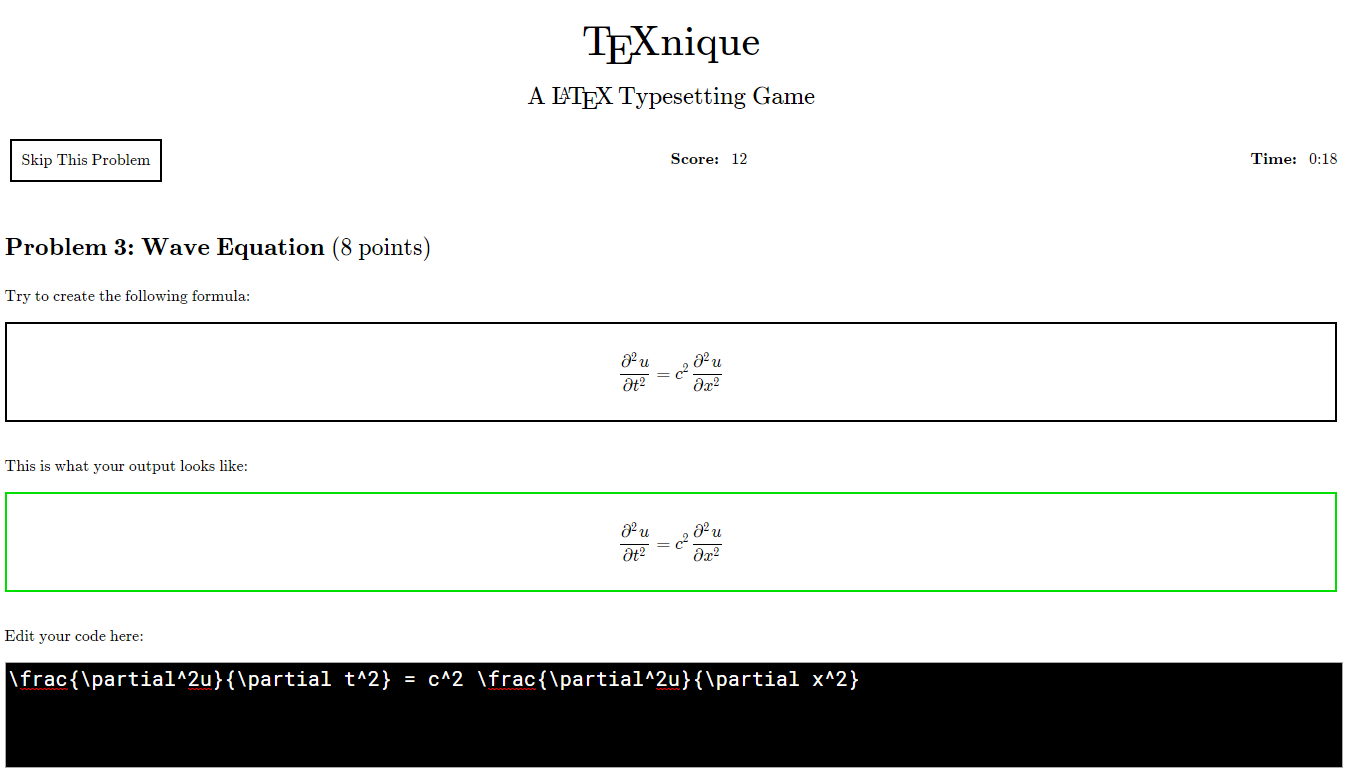
\includegraphics[width=1.0\linewidth,frame=]{./graphics/texnique.png}

% Caption is defined with a short and long version. The short version is shown in the 
% List of Figures section, and the long version is used directly with the figure. 			
	\caption[A screenshot of TeXnique, a game about typesetting equations.]{TeXnique, a game about typesetting equations \cite{texnique}. (Top) The game presents you with a rendered equation, (Bottom) the task is to enter LaTeX code that produces the same rendered equation. The green border on the lower rendering indicates it is a valid solution.}
	
% For figures label should be defined after the caption to ensure proper figure numbering.
	\label{fig:texnique}
\end{figure}
		
		TeXnique \cite{texnique} is web-browser based game for practising how to typeset equations in LaTeX. The game will present you with a rendered equation and your task is to type LaTeX code into the box below it such that your code produces the same (or closely matching / pixel equivalent) rendered equation. Figure \ref{fig:texnique} shows the game during play, the bottom rendered equation is bordered in green to indicate it is a valid match with the target. 

		% An example of how to center a passage of text, control local fontsize, 
		% and create a properly formatted and clickable URL.
		\begin{center}
		{\small \url{https://texnique.xyz}}
		\end{center}
		
		This is one of the more painful parts of typesetting a document, so it really takes a special kind of sadism to come up with such a game. Least to say, graduate students and researchers can be an odd bunch, and when we found this it was surprisingly addictive to compete over. 
		
		
		
	\section{Figures}
	\label{sec:typesetting_figures}
	
	In this template figures are numbered starting with the current chapter number followed by a figure number that resets to 1 each new chapter. As you can see below, the first figure is labelled Figure \ref{fig:dragon} because we are in Chapter \ref{chap:typesetting}.
	
	Figures in LaTeX are defined using a \lstinline|\begin{figure}...\end{figure}| environment and often immediately begin rendering in centre aligned mode by calling \lstinline|\centering|. Listing \ref{lst:latex_figure} below shows the LaTeX code used to typeset figure \ref{fig:dragon}. Figures \ref{fig:example_2x1} and \ref{fig:example_2x2} are defined similarly and make additional use of the \lstinline|\subfloat| command to position multiple images within a single figure environment, each with their own automatically incremented labels and individual captions.

	\lstinputlisting[label={lst:latex_figure}, caption={An example LaTeX excerpt demonstrating how to typeset figure \ref{fig:dragon} with a simple caption.}]{./listings/example_figure.tex}

	\subsection{Consistent presentation throughout the document}
		Figures work best in a document when you use a consistent style for formatting and captioning them and make sure that figures always actively support the content of the main text. 
	
	\subsection{Justified use of space in the document}
		All figures must be referred to directly in the main text of the document and discussed with meaningful and in depth critical analysis. If you don't need to use the figure to leverage and support your discussion then it is just taking up space and padding out the document. For example, you can use a command like \lstinline|\ref{fig:dragon}| to automatically get the figure number for Figure \ref{fig:dragon}. 	
		
		% [H] means put the figure HERE, directly when you input this code.
\begin{figure}[H]
	\centering

% We set the width of the figure based on the width of one line of text on the page. 
% The value can be tuned to any value in [0.0, 1.0] to scale the image while maintaining its aspect ratio.
	\includegraphics[width=1.0\linewidth]{./graphics/dragon.png}
	
% Caption is defined with a short and long version. The short version is shown in the 
% List of Figures section, and the long version is used directly with the figure. 		
	\caption[An image of many glass dragons being used to demonstrate typesetting a figure.]{A good caption should be sufficient enough to put the figure in context even if the reader has randomly flicked to the current page and looked only at the figure in isolation. All figures should also be referred to directly within the main text of your document. You can use the LaTeX \textbf{$\backslash$ref\{key\}} command to insert the correct figure number when you refer to it in the main text. By the very logic of this caption, this is a very poor caption because we still don't know why on earth is there an picture of glass dragons here. Image of glass dragons rendered using Path Tracing \cite{whittle15_dragons}.}
	
% For figures label should be defined after the caption to ensure proper figure numbering.
	\label{fig:dragon}
	
\end{figure}
		
	\subsection{Placement that supports and enhances the flow of the document}
		All figures shown in your document should be displayed in relevant locations, ideally just after that have been alluded to in the main text. Although there are many times where it is best to force a figure to the top or bottom of a nearby page.
	
	\subsection{Avoid directly importing other peoples images}
		You should avoid using other peoples figures whenever possible, and instead create your own figures for visualizing the specific methods and data you are working with in a way directly relevant to your project. 
	
	\subsection{Format sub-figures in LaTeX, not in the image itself}
		Construct sub-figures from multiple image files in LaTeX not in the image file itself. This allows you to tweak the positioning and layout without having to modify the images. It also allows for automatic formatting and numbering of captions and sub-captions. Figures \ref{fig:example_2x1} and \ref{fig:example_2x2} show examples of side-by-side and quad layouts respectively.
		
		% [H] means put the figure HERE, directly when you input this code.
\begin{figure}[H]
	\centering
	
% We use a figure width of 48.5% of the width of one line of text on 
% the page so there is some space between the images.
	\subfloat[Left image sub-caption.]{
		\includegraphics[width=0.485\linewidth]{./graphics/dragon.png}\label{fig:example_2x1_a}
	}~ % Use a tilde to add spacing for sub-figures that are displayed next to one another horizontally.
	\subfloat[Right image sub-caption.]{
		\includegraphics[width=0.485\linewidth]{./graphics/dragon.png}\label{fig:example_2x1_b}
	}\\ % New line before caption.

% Caption is defined with a short and long version. The short version is shown in the 
% List of Figures section, and the long version is used directly with the figure. 	
	\caption[A demonstration of a 2x1 sub-figure layout.]{Construct sub-figures from multiple image files in LaTeX not in the image file itself. This allows you to tweak the positioning and layout without having to modify the images. It also allows for automatic formatting and numbering of captions and sub-captions. Image of glass dragons rendered using Path Tracing \cite{whittle15_dragons}.}
	
% For figures label should be defined after the caption to ensure proper figure numbering.
	\label{fig:example_2x1}
	
\end{figure}
		
		% [H] means put the figure HERE, directly when you input this code.
\begin{figure}[H]
	\centering
	
% We use a figure width of 48.5% of the width of one line of text on 
% the page so there is some space between the images.
	\subfloat[Top-Left image sub-caption.]{
		\includegraphics[width=0.485\linewidth]{./graphics/dragon.png}\label{fig:example_2x2_a}
	}~ % Use a tilde to add spacing for sub-figures that are displayed next to one another horizontally.
	\subfloat[Top-Right image sub-caption.]{
		\includegraphics[width=0.485\linewidth]{./graphics/dragon.png}\label{fig:example_2x2_b}
	}\\ % New line before caption.
	\subfloat[Bottom-Left image sub-caption.]{
		\includegraphics[width=0.485\linewidth]{./graphics/dragon.png}\label{fig:example_2x2_c}
	}~ % Use a tilde to add spacing for sub-figures that are displayed next to one another horizontally.
	\subfloat[Bottom-Right image sub-caption.]{
		\includegraphics[width=0.485\linewidth]{./graphics/dragon.png}\label{fig:example_2x2_d}
	}\\ % New line before caption.
		
% Caption is defined with a short and long version. The short version is shown in the 
% List of Figures section, and the long version is used directly with the figure. 	
	\caption[A demonstration of a 2x2 sub-figure layout.]{A demonstration of a 2x2 sub-figure layout. Between A-B and C-D we use tilde symbols and between B-C we use a new line. Image of glass dragons rendered using Path Tracing \cite{whittle15_dragons}.}
	
% For figures label should be defined after the caption to ensure proper figure numbering.
	\label{fig:example_2x2}
	
\end{figure}
	
	\subsection{Robust captions that can stand in isolation}
		Figures need to be captioned such that they can be viewed in isolation and still be meaningful to the viewer. There will likely be some duplication of information that is written in the main text, but this is intended. 
	
	\subsection{Proper attribution and citation of images}
		\label{sec:typesetting_figures_citation}
		
		If an image does not belong to you it \textbf{must} be cited directly in the figure caption. \textbf{It is not correct to put a URL in the figure caption directly.} A URL in isolation is not an accurate or reliable way of directing a future reader to the exact content you are referencing. Instead make a new entry in your \lstinline|citations.bib| file and then reference that citation in the caption using the \lstinline|\cite{key}| command. Figures \ref{fig:dragon}, \ref{fig:example_2x1}, and \ref{fig:example_2x2} each include a statement in the caption stating ``Image of glass dragons rendered using Path Tracing \cite{whittle15_dragons}.''. When adding the BibTeX entry, try to find the proper information about the original author and source document to strengthen the citation in case the URL changes. 
	
	\section{Code Listings}
	\label{sec:typesetting_listings}
	
	Code listings should be formatted in the same style as figures and inline equations. It is important to use a monospace font so that characters line up vertically. Syntax highlighting is also extremely important for effectively displaying complicated code segments. To format inline code listings you can use the \lstinline[mathescape]|\lstinline$|$the_code$|$| command\footnote{So meta.}.
	
	% Longform Code listings should live in a code file, not embedded directly into your LaTeX code!
	\lstinputlisting[language={c}, label={lst:c_hello_world}, caption={An implementation of an important algorithm from our work.}]{./listings/hello_world.c}
	
	In LaTeX the ``Listings'' package can be used to properly format code and provide basic syntax highlighting, line numbering, and captioning of embedded code excerpts. Listing \ref{lst:listings} shows examples of how to properly format code using the listings package. 
	
	\newpage
	
	% Longform Code listings should live in a code file, not embedded directly into your LaTeX code!
	\lstinputlisting[label={lst:listings}, caption={Examples of methods for typesetting code listings within a LaTeX document.}]{./listings/listings.tex}
	
	\section{Tables}
	\label{sec:typesetting_tables}
	
	Tables are also quite predictably captioned and formatted the same way. It is important to decide on a style for how you will organize your data and apply that style consistently for all of your tables. Table \ref{tbl:example_table} shows one possible way of styling your data but is by no means the only way of doing so neatly. Consistency is the key. 
	
	% It's often a good idea to generate the LaTeX code for tables (python script or similar) so that if you rerun your code you don't have to typeset your results again by hand!
\begin{table}[H]
	\centering
	\scriptsize
	\caption[A demonstration of a table typeset in LaTeX.]{An example of a table formatted with caption.}
	
	% Tune the following two values that are being multiplied by the variable \textwidth
	% to control how large the scale of the table is, and how much is is squashed back 
	% to the final size.	
	\resizebox{0.8\textwidth}{!}{
		\begin{tabularx}{0.46\textwidth}{c|c|c|c|c|c}
			\toprule
			Some & Relevant & Fields & From & Your & Data\\
			\midrule
			0 & 0 & 0 & 0 & 0 & 0\\
			1 & 1 & 1 & 1 & 1 & 1\\
			2 & 2 & 2 & 2 & 2 & 2\\
			\bottomrule
		\end{tabularx}
		\label{tbl:example_table}
	}
\end{table}




	

	\chapter{Conclusions and Future Work}
\label{chap:conclusion}

In this document we have demonstrated the use of a LaTeX thesis template which can produce a professional looking academic document. 

\section{Contributions} 
\label{sec:conclusion_contributions}

The main contributions of this work can be summarized as follows:
\begin{description}	

	\item[$\bullet$ A LaTeX thesis template]\hfill
	
	Modify this document by adding additional top level content chapters. These descriptions should take a more retrospective tone as you include summary of performance or viability. 
	
	
	\item[$\bullet$ A typesetting guide of useful primitive elements]\hfill
	
	Use the building blocks within this template to typeset each part of your document. Aim to use simple and reusable elements to keep your document neat and consistently styled throughout.
	
	\item[$\bullet$ A review of how to find and cite external resources]\hfill
		
	We review techniques and resources for finding and properly citing resources from the prior academic literature and from online resources. 
	
\end{description}

\section{Future Work}
\label{sec:conclusion_future_work}

Future editions of this template may include additional references to Futurama.
	
% Formatting citations properly when they are rendering incorrectly in your PDF can be fiddly,
% espectially when punctuation and international characters are involed. Sometimes multiple re-compilations
% are needed in addition to clearing temporary auxiliary files to see your changes in your document.
% Insert the bibliography using citations contained in the file citations.bib
	\bibintoc%
	\bibliography{citations} 
	
% In the appendix you might include a full code listing for an implemented algorithm that you showed a 
% small chunk of in one of your chapters. If you have extra graphs for ablation style experiments you 
% might enumerate them within the appendix and use \label{name} and \ref{name} to automatically insert 
% the correct section locations when you talk about them in your chapters.
% Within appendix.tex you should use chapters as the top level section dividers.
	\appendix
	\addappheadtotoc
	\chapter{Implementation of a Relevant Algorithm}
\label{app:implementation_algorithm}

% Code listings should live in a code file, not embedded directly into your LaTeX code!
\lstinputlisting[language=c, label={lst:c_hello_world}, caption={An implementation of an important algorithm from our work.}]{./listings/hello_world.c}

\chapter{Supplementary Data}
\label{app:supplementary_data}

The results of large ablative studies can often take up a lot of space, even with neat visualization and formatting. Consider putting full results in an appendix chapter and showing excerpts of interesting results in your chapters with detailed analysis. You can use labels and references to refer the reader here for the full data.

	
\end{document}